\documentclass[11pt]{article}
\usepackage[margin=1in]{geometry}
\usepackage{amsmath,amssymb,amsthm}
\usepackage{booktabs}
\usepackage[hidelinks]{hyperref}
\usepackage{xcolor}
\usepackage{graphicx}
% Shared notation for the differential-geometric SN Ia light-curve project.
% Input this file from every scientific document so notation stays consistent.
%
% Requires: amsmath, amssymb

% --- Number sets -------------------------------------------------------
\newcommand{\Real}{\mathbb{R}}
\newcommand{\Rn}{\mathbb{R}^{n}}
\newcommand{\Rtwo}{\mathbb{R}^{2}}
\newcommand{\Rthree}{\mathbb{R}^{3}}

% --- Differential geometry ---------------------------------------------
\newcommand{\dd}{\mathrm{d}}
\newcommand{\curve}{\gamma}                 % the light-curve curve
\newcommand{\arc}{s}                        % arclength
\newcommand{\curv}{\kappa}                  % curvature
\newcommand{\tors}{\tau}                    % torsion (n >= 3 only); unused in the note,
                                            % where bare \tau is the coefficient-prior scale
\newcommand{\frenet}[1]{\mathbf{E}_{#1}}    % Frenet frame vector
\newcommand{\tang}{\mathbf{T}}              % unit tangent
\newcommand{\norml}{\mathbf{N}}             % unit normal
\newcommand{\arcmax}{\arc_{\max}}           % upper end of the arclength interval;
                                            % NOT its length, which is arcmax - arcmin

% --- Model parameters ---------------------------------------------------
\newcommand{\allpars}{\Theta}               % ALL per-SN parameters; \shape is the
                                            % subset that conditions \curv
\newcommand{\shape}{\theta}                 % shape latents
\newcommand{\shapeone}{\theta_{1}}
\newcommand{\shapetwo}{\theta_{2}}
\newcommand{\tscale}{w}                     % timing scale (rest-frame days);
                                            % NOT \sigma, which is reserved for
                                            % flux measurement errors
\newcommand{\tmax}{t_{\mathrm{max}}}        % time origin
\newcommand{\stretchsym}{\varsigma}         % classical stretch factor (Phillips/Goldhaber,
                                            % SALT2 s); deliberately NOT \arc, which is arclength
\newcommand{\warpone}{a_{1}}                % quadratic timing corrections
\newcommand{\warptwo}{a_{2}}
\newcommand{\peakmag}{m_{g}^{\max}}         % FITTED apparent peak g magnitude; absorbs
                                            % absolute magnitude, distance and grey offsets
\newcommand{\dm}{\mu}                       % distance modulus -- extracted downstream by
                                            % standardization, NOT the fitted normalization
\newcommand{\colr}{c}                       % colour amplitude (variant only)
\newcommand{\xstretch}{x_{s}}               % per-SN phase dilation (SALT2 x_1 analogue);
                                            % NOT \stretch, a LaTeX primitive
\newcommand{\shapeturn}{x_{\psi}}          % per-SN shape coefficient; multiplies the
                                            % turning mode Psi_1, not a curvature
\newcommand{\turnzero}{\Psi_{0}}            % reference turning, an angle not a curvature
\newcommand{\turnone}{\Psi_{1}}             % first mode of departure in turning
\newcommand{\dustunit}{\hat{\mathbf{e}}_{\colr}}  % reddening DIRECTION, a unit vector;
                                            % \dustdir is the phase-dependent displacement
\newcommand{\dustdir}{\mathbf{u}}           % phase-dependent reddening
                                            % displacement, u(s); NOT a constant, and NOT
                                            % the scalar u = asinh(s/delta) of the note

% --- Photometry ---------------------------------------------------------
\newcommand{\magg}{m_{g}}                   % observed/predicted magnitude, band g
\newcommand{\magr}{m_{r}}
\newcommand{\Magg}{M_{g}}                   % TEMPLATE magnitude, band g; NOT \magg
\newcommand{\Magr}{M_{r}}
\newcommand{\fluxg}{f_{g}}
\newcommand{\fluxr}{f_{r}}
\newcommand{\zp}{\mathrm{zp}}
\newcommand{\phase}{p}                      % rest-frame phase
\newcommand{\zred}{z}

% --- Objects and abbreviations -----------------------------------------
\newcommand{\snia}{SN\,Ia}
\newcommand{\sneia}{SNe\,Ia}
\newcommand{\ztf}{ZTF}
\newcommand{\salt}{SALT2}

% --- Operators ----------------------------------------------------------
\DeclareMathOperator{\sign}{sign}
\DeclareMathOperator{\asinh}{asinh}
\DeclareMathOperator{\SO}{SO}
\DeclareMathOperator{\SE}{SE}
\DeclareMathOperator*{\argmin}{arg\,min}
\newcommand{\deriv}[2]{\frac{\dd #1}{\dd #2}}
\newcommand{\pderiv}[2]{\frac{\partial #1}{\partial #2}}
\newcommand{\abs}[1]{\left| #1 \right|}
\newcommand{\norm}[1]{\left\| #1 \right\|}


\newcommand{\file}[1]{\texttt{#1}}
\newcommand{\code}[1]{\texttt{#1}}

\title{What the Code Implements}
\author{read out of \file{stan/} and \file{src/dgsn/stan/}}
\date{\today}

\begin{document}
\maketitle

\noindent
\file{model-definition.tex} says what the model should be. This says what the code does. It
is written from \file{stan/} and \file{src/dgsn/stan/data.py} and not from that note, so
that the two can be compared and any divergence seen rather than assumed away. Every
statement below names the file and function it comes from.

\paragraph{How to read the correspondence.} Each implemented piece is tagged with where it
comes from in the note. Equation and section numbers are the note's own.
\begin{itemize}
\item[\textbf{[=]}] \emph{As written.} The code evaluates the note's equation directly.
\item[\textbf{[+]}] \emph{Fused.} The code evaluates a single expression that the note states
  across two or more places --- usually a defining equation in Section~2 together with a
  change of variable or a Jacobian recorded in Section~5.1. These are not divergences, but
  they are where a reader of one section alone can form the wrong expectation, and
  Section~\ref{sec:fused} says so explicitly.
\item[\textbf{[c]}] \emph{Construction.} The note states a property; the code obtains it by
  how it builds the basis rather than by imposing a condition, so the property holds
  identically and there is nothing to check at run time.
\item[\textbf{[!]}] \emph{Divergent.} The code and the note disagree. Collected in
  Section~\ref{sec:differ}.
\item[\textbf{[0]}] \emph{Not in the note.} Machinery with no counterpart there.
\end{itemize}

\section{The programs}

One \code{functions} block, \file{stan/dgsn\_functions.stan}, is \code{\#include}d by every
program; the grid declarations are \file{dgsn\_grid\_data.stan} in a \code{data} block and
\file{dgsn\_grid\_tdata.stan} in a \code{transformed data} block. Nothing per-supernova is
hard-coded: every constant arrives as data from \file{src/dgsn/stan/data.py}.

\begin{tabular}{llll}
\toprule
program & samples & purpose & \\
\midrule
\file{hier.stan}        & the hierarchy & Section~5, stages 3 and 4 & \textbf{[=]} \\
\file{hier\_nomode.stan} & the hierarchy with $\shapeturn \equiv 0$ & whether the turning mode earns its place & \textbf{[0]} \\
\file{hier\_common.stan} & also with $x_p \equiv 0$ & whether either does & \textbf{[0]} \\
\file{single\_sn.stan}  & one supernova, globals as data & Section~5.2, stage 2 & \textbf{[=]} \\
\file{track\_fit.stan}  & one track, no priors & \salt\ floors, Section~5.2 & \textbf{[=]} \\
\file{forward.stan}     & nothing (\code{fixed\_param}) & the forward map for diagnostics & \textbf{[=]} \\
\file{jacobian.stan}    & nothing (\code{fixed\_param}) & log fluxes, for the Fisher information & \textbf{[0]} \\
\file{checks.stan}      & nothing (\code{fixed\_param}) & closed-form quadrature tests & \textbf{[=]} \\
\bottomrule
\end{tabular}

\section{The forward map}

\code{log\_flux} in \file{dgsn\_functions.stan} takes an epoch's $\Delta t$ and band and
returns four columns: log flux, log taper, arclength before the clamp, arclength after. It
runs in four steps, which assemble Eqs.~(7), (8), (10), (17) and (19)--(20) of the note.

\paragraph{Phase, clamped. [+] Eq.~(7) with Eq.~(19).} With $\Delta$ the offset and
$\zred$ known,
\begin{equation}
  w_{i} = \frac{(\Delta t_{i} - \Delta)/(1 + \zred) - \phase_{\min}}
               {\phase_{\max} - \phase_{\min}} , \qquad
  \hat\phase_{i} = \phase_{\min} + (\phase_{\max} - \phase_{\min})\,
    \mathrm{clamp01}(w_{i}, \epsilon) ,
\end{equation}
which is Eq.~(7)'s $\phase = (t - \tmax)/(1 + \zred)$ with $\tmax = t_{0} + \Delta$,
composed with the clamp of Eq.~(19): $\mathrm{clamp01}(w, \epsilon) =
\mathrm{softplus}(w, \epsilon) - \mathrm{softplus}(w - 1, \epsilon)$ and
$\mathrm{softplus}(x, \epsilon) = \epsilon\log(1 + e^{x/\epsilon})$, written branch-free so
that neither limb overflows --- an implementation detail with no counterpart in the note,
and algebraically identical to it. The taper is
$\log\mathcal{T}_{i} = -[e_{i}/\epsilon_{t}]^{2}$ with
$e_{i} = \mathrm{softplus}(-w_{i}, \epsilon_{t}/10) +
\mathrm{softplus}(w_{i} - 1, \epsilon_{t}/10)$, so it is evaluated at the \emph{unclamped}
$w$ and turns the flux off outside the window.

\paragraph{Arclength, clamped. [+] Eq.~(10) with Eq.~(12), Section~5.1's Jacobian, and
Eq.~(20).} \code{arclength} integrates
\begin{equation}
  \arc(\phase) = e^{\xstretch}\!\int_{0}^{\phase}
    \exp[q_{0} + x_p q_{1}]\,\delta_{p}\cosh v\,\dd v ,
\end{equation}
which is the \emph{one} place three of the note's statements are fused, and the fusion is
worth naming. Eq.~(10) gives $\dd\arc/\dd\phase = \exp[\xstretch + q_{0} + x_p q_{1}]$ with
$\arc(\phase) = \int_{0}^{\phase}$, an integral in $\dd\phase$. Eq.~(12) gives
$v = \asinh(\phase/\delta_{p})$ with $\delta_{p} = 1$~d. And Section~5.1 --- four sections
later, in prose rather than an equation --- supplies $\dd\phase = \delta_{p}\cosh v\,\dd v$.
The code integrates over fixed $v$ nodes with the weights already multiplied by that
Jacobian, \code{jacw\_v}, so the expression above is what it evaluates and no single
equation of the note matches it. $\xstretch$ leaves the integral as a multiplicative
$e^{\xstretch}$, and the coefficient vector passed in is
$\mathbf{b} + x_p\mathbf{a}$. Then the clamp of Eq.~(20) with $\epsilon_{s}$ onto
$[\arc_{\min}, \arcmax]$.

\paragraph{The curve. [+] Eq.~(5) with Eqs.~(9), (14) and Section~5.1's Jacobian.}
\code{curve} integrates
$\curve(\arc) = \int_{0}^{\arc}(\cos\psi, \sin\psi)\,\delta\cosh u\,\dd u$ with
$\psi(u) = -\pi/2 + \tilde{\mathbf{P}}(u)\cdot(\mathbf{d} + \shapeturn\mathbf{c})$, at the
clamped $\hat\arc$. The same three-way fusion as the traversal: Eq.~(5) for the integral,
Eq.~(9) for $\psi$, Eq.~(14) for $u = \asinh(\arc/\delta)$, and Section~5.1 for
$\dd\arc = \delta\cosh u\,\dd u$. Here, and unlike the traversal, the note's gauge is
written in the same measure the integral carries --- see Section~\ref{sec:gauge}.

\paragraph{Magnitudes and flux. [=] Eqs.~(8) and (17).} Band $1$ is $g$, band $2$ is
$r$:
\begin{equation}
  \magg = \curve_{1} + \peakmag , \qquad \magr = \curve_{2} + \peakmag - \colr ,
  \qquad
  \log \hat f_{i} = -0.4\ln 10\,(m_{b_{i}} - \zp) + \log\mathcal{T}_{i} .
\end{equation}
The two basis vectors of magnitude space are therefore $(1,1)$ for $\peakmag$ and $(0,-1)$
for $\colr$, as coefficients and not as a rotation.

\section{The two bases}
\label{sec:bases}

Eqs.~(13) and (15) of the note give the expansions; the orthonormality each one satisfies is
a property of how the code builds it.

\code{legendre\_row} returns degrees $0$ to $n-1$ on $[lo, hi]$, each scaled by
$\sqrt{(2k+1)/(hi-lo)}$, so the set is orthonormal under $\int fg\,\dd x$ over that
interval.

\paragraph{Traversal. [c] Eq.~(13).} \code{traversal\_row} is
\code{legendre\_row(v, Kq, vlo, vhi)[2:Kq]}:
degrees $1$ to $K_{q}-1$ in $v$, the constant dropped. Orthonormality in $v$ and the absence
of a constant are therefore properties of the basis, so $\bar q_{0} = \bar q_{1} = 0$ and
$\langle q_{j}, q_{k}\rangle = \delta_{jk}$ hold identically and are not imposed. Eq.~(11)
lists four gauge conditions; two of them, $\bar q_{0} = 0$ and $\bar q_{1} = 0$, are these,
so the code imposes two and inherits two. One consequence: $q_{0}$ \emph{cannot} carry a
constant, which is why the mean log rate has to live in $\xstretch$ --- Eq.~(22).

\paragraph{Turning. [c] Eq.~(15) with Eq.~(9)'s condition at the anchor.}
\code{turning\_row} is
$[\mathbf{P}(u)_{1:K_{\psi}-1} - \mathbf{P}(0)_{1:K_{\psi}-1}]\,T$: Legendre in $u$ with the
constant dropped, shifted to vanish at $u = 0$, then re-orthonormalized by $T$, the
transpose-inverse of the Cholesky factor of $I + (u_{\mathrm{hi}} - u_{\mathrm{lo}})
\mathbf{P}(0)^{\mathsf T}\mathbf{P}(0)$. $T$ is upper triangular, so mode $k$ mixes degrees
at most $k$. Hence $\turnzero(0) = \turnone(0) = 0$ --- Eq.~(9)'s own side condition --- holds by
construction rather than by a fitted constraint, and the basis is orthonormal in $u$,
\emph{not} in $\arc$. That last fact is where the gauge and the basis part company, below.

\section{The gauge}
\label{sec:gauge}

Eq.~(11) of the note. Four conditions for four freedoms, of which the code imposes two per
pair and inherits the means from the bases of Section~\ref{sec:bases}.

In \file{hier.stan}, \code{transformed parameters}:
\begin{equation}
  \tilde{\mathbf{a}} = k^{-(\alpha_{q}-\frac12+\frac12)}\mathbf{z}_{a} , \quad
  \mathbf{a} = \frac{\tilde{\mathbf{a}}}{\lVert\tilde{\mathbf{a}}\rVert} , \quad
  \mathbf{b} = \tilde{\mathbf{b}} - (\tilde{\mathbf{b}}\!\cdot\!\mathbf{a})\,\mathbf{a} ,
\end{equation}
\begin{equation}
  \tilde{\mathbf{c}} = k^{-(\alpha_{\psi}-\frac12+\frac12)}\mathbf{z}_{c} , \quad
  \mathbf{c} = \frac{\tilde{\mathbf{c}}}{\sqrt{\tilde{\mathbf{c}}^{\mathsf T}
    G_{\arc}\tilde{\mathbf{c}}}} , \quad
  \mathbf{d} = \tilde{\mathbf{d}} - (\tilde{\mathbf{d}}^{\mathsf T}G_{\arc}\mathbf{c})\,
    \mathbf{c} .
\end{equation}
\paragraph{The traversal pair. [=] Eq.~(11) as written.} The code uses the plain Euclidean
inner product on coefficients, which \emph{is} $\int fg\,\dd v$ because the basis is
orthonormal in $v$. So $\langle q_{1},q_{1}\rangle = 1$ reads
$\lVert\mathbf{a}\rVert = 1$, and the fits give $1.0000 \pm 0.0000$.

\paragraph{The turning pair. [=] Eq.~(11), in the measure Eq.~(11) asks for.} $G_{\arc}$ is
built by \code{turning\_gram\_s} as
$\int \tilde P_{j}\tilde P_{k}\,\delta\cosh u\,\dd u$ over the gauge span, on its own
two-sided rule of $200$ panels a side rather than the $m$ of the run. Because the basis is
orthonormal in $u$ and not in $\arc$, $G_{\arc} \neq I$: measured, its eigenvalues run
$4.55$ down to $1.65\times10^{-5}$. So $\mathbf{c}^{\mathsf T}G_{\arc}\mathbf{c} = 1$ fixes
$\lVert\mathbf{c}\rVert$ only through its direction, and the fits give $1.353 \pm 0.213$ at
$(12, 8)$ and $0.806 \pm 0.171$ at $(24, 16)$. $\mathbf{b}$ and $\mathbf{d}$ carry whatever
norm the data give them, there being no parameter beside them to absorb a rescaling.

\paragraph{The asymmetry this leaves.} The note argues in Section~2.3 that the turning
product must be taken in $\arc$ and not in the expansion coordinate $u$, since a mode of
unit $u$-norm can carry its power where $\dd\arc$ is small and the curve, an integral
$\dd\arc$, cannot see it. The same argument applies to the traversal with $\phase$ for
$\arc$ and $v$ for $u$ --- Eq.~(10) integrates in $\dd\phase$ --- but Eq.~(11) specifies
that pair in $\dd v$. The two measures disagree by a factor of $45$ in Jacobian, and
measured on the fitted mode at a single draw, $\int q_{1}^{2}\,\dd v = 1.000$ against
$\int q_{1}^{2}\,\dd\phase = 12.6$ to $15.2$. The code follows Eq.~(11) exactly; the
asymmetry is the note's, and is recorded here because the code is where it shows.

In \file{hier\_nomode.stan} there is no $\mathbf{c}$: $\mathbf{d} = \tilde{\mathbf{d}}$, the
turning pair has no gauge, and $\mathbf{c} = \mathbf{0}$ and $\shapeturn = 0$ are
\code{transformed data} constants.

\section{The grid}

Section~5.1 of the note. \textbf{[=]} in structure, \textbf{[!]} in one constant.

\file{dgsn\_grid\_tdata.stan} lays, in each of $u$ and $v$, $m$ equal panels on $[lo, 0]$ and
$m$ on $[0, hi]$, a $J$-point Gauss--Legendre rule in each, so zero is edge $m+1$ of
$2m+1$. Weights are stored already multiplied by their Jacobians,
$\delta\cosh u$ and $\delta_{p}\cosh v$. \code{prefix\_from\_zero} accumulates panel
integrals outward from zero, giving $C[m+1] = 0$ exactly; an epoch's remainder past the last
edge is one further fresh $J$-point panel on $[e_{0}, x]$. \code{panel\_of} finds the panel
by a comparison loop rather than \code{floor}, which Stan will not cast when the argument
depends on parameters.

\section{The likelihood}

Eq.~(18) of the note, with the tapered flux of Eq.~(17). \textbf{[=]}

\code{neg2\_loglike}, over all epochs, on the archive's errors alone:
\begin{equation}
  -2\ln\mathcal{L} = \sum_{i}
    \frac{(f_{i} - \hat f_{i})^{2}}{\sigma_{f,i}^{2}} .
\end{equation}
$\hat f_{i}$ is the \emph{tapered} flux, so an epoch outside the window has its residual
suppressed. In \file{hier.stan} the sum is a \code{reduce\_sum} over supernovae with the
slice width passed as \code{grainsize}. The function takes
$(\mathbf{f}, \boldsymbol{\sigma}_{f}, \hat{\mathbf{f}})$ and nothing else: the band index
went with the per-band scatter it used to select.

\section{The hierarchy}

Section~5 of the note. The priors are its Eq.~(21) on the coefficients and the per-supernova
statements of Section~5; Eq.~(22) is the parameterization of $\xstretch$.

\begin{tabular}{llll}
\toprule
sampled & shape & prior & reaches the map as \\
\midrule
\code{w\_coef}      & $2(K_{q}{-}1) + 2(K_{\psi}{-}1)$ & see below & $\mathbf{raw} = R\,\code{w\_coef}$ \\
\code{tau\_q}, \code{tau\_psi}       & scalar $>0$ & flat & scale of $\tilde{\mathbf{b}}, \tilde{\mathbf{d}}$ \\
\code{alpha\_q\_m}, \code{alpha\_psi\_m} & scalar $>0$ & $\mathrm{Exp}(1)$ & $\alpha - \frac12$ \\
\code{sigma\_g}, \code{sigma\_r}     & scalar $>0$ & flat & the scatters \\
\code{mu\_p}, \code{mu\_psi}, \code{mu\_delta} & scalar & flat & locations \\
\code{s\_delta}     & scalar $>0$ & flat & scale of $\Delta$ \\
\code{s\_bar}       & scalar & $\mathcal{N}(0, 10^{2})$ & mean of $\xstretch$ \\
\code{x\_s\_dev}    & \code{sum\_to\_zero\_vector}$[N]$ & $\mathcal{N}(0,1)$ & $\xstretch = \code{s\_bar} + \code{x\_s\_dev}$ \\
\code{m\_peak}      & $N$ & $\mathcal{N}(m_{g}^{\mathrm{bright}}, 1)$ & $\peakmag$ \\
\code{colr}         & $N$ & $\mathcal{N}(0,1)$ & $\colr$ \\
\code{u\_p}         & $N$ & $\mathcal{N}(0,1)$ & $x_p = \code{mu\_p} + \code{u\_p}$ \\
\code{u\_psi}       & $N$ & $\mathcal{N}(0,1)$ & $\shapeturn = \code{mu\_psi} + \code{u\_psi}$ \\
\code{u\_del}       & $N$ & $\mathcal{N}(0,1)$ & $\Delta = \code{mu\_delta} + \code{s\_delta}\,\code{u\_del}$ \\
\bottomrule
\end{tabular}

\medskip\noindent
\code{w\_coef} is sliced, after the rotation, into
$\mathbf{z}_{a}, \tilde{\mathbf{b}}, \mathbf{z}_{c}, \tilde{\mathbf{d}}$, with
$\mathbf{z}_{a}, \mathbf{z}_{c}$ standard normal and
\begin{equation}
  \tilde b_{k} \sim \mathcal{N}\!\left(0,\;
    \tau_{q}\,(k/\bar k_{q})^{-(\alpha_{q}-\frac12+\frac12)}\right) ,
\end{equation}
and likewise $\tilde{\mathbf{d}}$, where $\bar k = \exp[\overline{\ln k}]$ is the
geometric-mean mode. So $\tau$ is the scale of a mid-range mode, and it informs only the
centred pair: the gauge removes the scale of $\mathbf{a}$ and $\mathbf{c}$ entirely.

The two simplified programs are Section~\ref{sec:nested}.

\paragraph{The rotation.} $R$ is a square \code{data} matrix over the coefficient block,
identity unless a preconditioner has been built. Since it is constant its Jacobian is
constant, so it changes no posterior. \file{src/dgsn/stan/precondition.py} builds it as
$R = L^{-\mathsf T}$ with $LL^{\mathsf T}$ the Fisher information
$J^{\mathsf T}\Sigma^{-1}J$ plus the prior precision, $J$ differenced from
\file{jacobian.stan} so that the gauge is the fit's own.

\paragraph{Relabeling.} \code{generated quantities} reports the sign branches
$\code{flip\_q} = [\int_{0}^{v_{\max}} q_{1}\,\dd v < 0]$ and
$\code{flip\_psi} = [\turnone(\arc_{\mathrm{g}+}) < 0]$, and the relabeled
$\mathbf{a}_{\mathrm{rel}}, \mathbf{c}_{\mathrm{rel}}, x_{p,\mathrm{rel}},
x_{\psi,\mathrm{rel}}$. It also reports \code{lp\_sn} per supernova,
$\arc$ at the window ends, and the tapered and clamped fractions.

\section{The nested hierarchies}
\label{sec:nested}

\textbf{[0]} --- neither program is in the note. Each removes a departure mode of
Section~2.3, and what goes with a mode is more than its term.

\begin{tabular}{llll}
\toprule
 & \file{hier.stan} & \file{hier\_nomode.stan} & \file{hier\_common.stan} \\
\midrule
turning, Eq.~(9)        & $-\frac{\pi}{2} + \turnzero + \shapeturn\turnone$
                        & $-\frac{\pi}{2} + \turnzero$
                        & $-\frac{\pi}{2} + \turnzero$ \\
traversal, Eq.~(10)     & $\xstretch + q_{0} + x_p q_{1}$
                        & $\xstretch + q_{0} + x_p q_{1}$
                        & $\xstretch + q_{0}$ \\
\code{w\_coef} length   & $2(K_{q}{-}1) + 2(K_{\psi}{-}1)$
                        & $2(K_{q}{-}1) + (K_{\psi}{-}1)$
                        & $(K_{q}{-}1) + (K_{\psi}{-}1)$ \\
coefficients at $(24,16)$ & 76 & 53 & 38 \\
sampled values, $N = 30$  & 267 & 213 & 167 \\
per supernova           & 6 & 5 & 4 \\
gauge conditions        & 4 on $q$, 2 on $\psi$ & 4 on $q$ & \emph{none} \\
sign conventions        & \code{flip\_q}, \code{flip\_psi} & \code{flip\_q} & \emph{none} \\
cost per \code{log\_prob} & $0.097$~s & $0.084$~s & $0.113$~s \\
\bottomrule
\end{tabular}

\paragraph{How a mode is removed.} Not by setting its coefficients to zero, which the gauge
forbids: $\mathbf{a} = \tilde{\mathbf{a}}/\lVert\tilde{\mathbf{a}}\rVert$ is undefined there.
The mode vector and its amplitudes are held at zero as \code{transformed data} constants ---
\code{a\_zero}, \code{c\_zero}, \code{x\_p\_zero}, \code{x\_psi\_zero} --- so they cost
nothing per draw and no dead column reaches the output, and the shared \code{functions}
block needs no change at all, taking the combined $\mathbf{d} + \shapeturn\mathbf{c}$ and
$\mathbf{b} + x_p\mathbf{a}$ as it already did. The parameters that go with the mode are its
amplitudes and their location: \code{mu\_psi} and \code{u\_psi} with $\turnone$,
\code{mu\_p} and \code{u\_p} with $q_{1}$.

\paragraph{The gauge empties.} Every condition in Eq.~(11) names a mode. $\bar q_{1} = 0$
and $\langle q_{1},q_{1}\rangle = 1$ are conditions \emph{on} $q_{1}$;
$\langle q_{0},q_{1}\rangle = 0$ and $\bar q_{0} = 0$ fix $q_{0}$'s component along $q_{1}$
and its constant, and the constant is already absent from the basis. So in
\file{hier\_common.stan} the \code{transformed parameters} block reads
$\mathbf{b} = \tilde{\mathbf{b}}$ and $\mathbf{d} = \tilde{\mathbf{d}}$, nothing is
normalized, and $G_{\arc}$ --- still built in \code{transformed data}, the include being
shared --- is never used. $q_{0}$ and $\turnzero$ are functions the data determine outright,
with no coordinate freedom left to fix.

\paragraph{And so do the sign conventions.} The two freedoms of Section~2.3 are
$(q_{1}, x_p) \mapsto (-q_{1}, -x_p)$ and $(\turnone, \shapeturn) \mapsto
(-\turnone, -\shapeturn)$, each belonging to a mode. \file{hier\_common.stan} has neither, so
it reports no \code{flip\_q}, no \code{flip\_psi}, and none of
$\mathbf{a}_{\mathrm{rel}}, \mathbf{c}_{\mathrm{rel}}, x_{p,\mathrm{rel}},
x_{\psi,\mathrm{rel}}$: every quantity it writes is already in one branch. That removes by
construction a defect rather than a nuisance --- a relabeling read off the sign of
$\turnone$ at one point is unstable when $\turnone$ has a node there, and such a relabeling
contaminated \code{R-hat} on $\mathbf{c}_{\mathrm{rel}}$ in the fits that have one.

\paragraph{What stays.} \code{tau\_q}, \code{alpha\_q\_m}, \code{tau\_psi} and
\code{alpha\_psi\_m} are the prior scale and decay of $\tilde{\mathbf{b}}$ and
$\tilde{\mathbf{d}}$ by Eq.~(21), which are $q_{0}$'s and $\turnzero$'s own expansions and
have nothing to do with the modes. In \file{hier.stan} $\tau_{q}$ informs only the centred
pair, the gauge having removed $\mathbf{a}$'s scale; here there is no $\mathbf{a}$ to
remove a scale from, so $\tau_{q}$ simply is $q_{0}$'s scale.

\paragraph{They are nested, and the embedding is exact.} A mode reaches the likelihood only
through its amplitude, so a point of the simpler model is a point of the richer one with the
new amplitudes at zero: $\mathbf{b} + x_p\mathbf{a}$ reduces to $\mathbf{b}$ whatever
$\mathbf{a}$ is. \code{hier\_data.inits\_from\_run} does that, which makes a simpler fit's
posterior a start for the next rung --- a point a sampler has occupied, rather than a
template's or an optimizer's. Two cautions found in building it. The start must be taken
from a \emph{draw}, not from the mean of the draws: the model is nonlinear, so a
parameter-wise mean need not be a point the model fits, and on an unconverged source it is
not, costing $21000$ nats where a draw transfers to the digit. And a source with chains in
both sign branches must be relabeled first, in the blocks
$\mathbf{z}_{a}, \tilde{\mathbf{b}}, \mathbf{z}_{c}, \tilde{\mathbf{d}}$ rather than in
\code{w\_coef}: $R$ mixes \code{w\_coef}'s slots, so negating one is wrong, and a point
built from an unrelabeled \code{w\_coef} beside a relabeled \code{mu\_p} has
$\mathbf{a}$'s sign against $x_p$'s, which inverts the traversal.

\paragraph{What removing each mode costs.} At the optimum, on thirty supernovae at
$(24, 16)$: $-13258.5$ with both modes, $-13271.9$ without $\turnone$, $-13432.0$ without
either. So $\turnone$ is worth $13$ nats and $q_{1}$ a further $160$ --- $q_{1}$ about twelve
times $\turnone$, which inverts what the sampling diagnostics suggest and agrees with them:
$\turnone$ is the badly determined mode, four informed directions of $23$ falling as
$k^{-2.79}$, and being well determined is what makes a mode expensive to remove.

\section{\file{hier\_common.stan} in full}
\label{sec:common}

Self-contained: this section repeats in particular what the sections above give in general,
so that the simplest program can be read without them. Everything here is the code's, taken
from \file{stan/hier\_common.stan} and the \code{functions} block it includes.

\subsection{What the model says}

Every supernova walks one curve in magnitude space at one rate profile, and differs from
every other only in where it is placed, how fast it goes, and when. For supernova $n$
observed at time $t$, with redshift $\zred_{n}$ known and $t_{0,n}$ the archive's \salt\
time of $B$ maximum:
\begin{align}
  \phase &= \frac{t - t_{0,n} - \Delta_{n}}{1 + \zred_{n}} ,
    \label{eq:cphase}\\
  \deriv{\arc}{\phase} &= \exp\bigl[x_{s,n} + b_{0}P_{0} + q_{0}(\phase)\bigr] ,
    \qquad \arc(0) = 0 ,\ \textstyle\sum_{n} x_{s,n} = 0 ,
    \label{eq:ctrav}\\
  \psi(\arc) &= -\frac{\pi}{2} + \turnzero(\arc) , \qquad \turnzero(0) = 0 ,
    \label{eq:cturn}\\
  \curve(\arc) &= \int_{0}^{\arc}\bigl(\cos\psi,\ \sin\psi\bigr)\,\dd\arc' ,
    \qquad \curve(0) = 0 ,
    \label{eq:ccurve}\\
  \begin{pmatrix} \magg \\ \magr \end{pmatrix} &=
    \curve\bigl(\arc(\phase)\bigr) + m_{g,n}^{\max}\begin{pmatrix} 1 \\ 1 \end{pmatrix}
    + \colr_{n}\begin{pmatrix} 0 \\ -1 \end{pmatrix} ,
    \label{eq:cmag}\\
  \hat f &= 10^{-0.4\,(m_{b} - \zp)}\,\mathcal{T} .
    \label{eq:cflux}
\end{align}
$q_{0}$ and $\turnzero$ are shared by every supernova; $m_{g,n}^{\max}, \colr_{n}, x_{s,n},
\Delta_{n}$ are its own. $\mathcal{T}$ is the taper of \S\ref{sec:csoft}. Nothing else
varies: there is no per-supernova freedom in the \emph{shape} of either the curve or the
rate.

\paragraph{Three conditions at the anchor, and what they buy.} $\arc(0) = 0$,
$\turnzero(0) = 0$ and $\curve(0) = 0$ all hold at $\phase = 0$, the last of them because
\eqref{eq:ccurve} integrates from zero. Taken together they pin the anchor completely: at
$\phase = 0$ the arclength is zero, the curve is at the origin of the $(\magg, \magr)$
plane in \emph{both} components, and \eqref{eq:cmag} therefore reads
$(\magg, \magr) = (m_{g,n}^{\max},\, m_{g,n}^{\max} - \colr_{n})$. That is what makes
$m_{g}^{\max}$ the $g$ magnitude and $\colr$ the $g-r$ colour there rather than some
combination, and $\psi(0) = -\pi/2$ adds that the curve leaves the origin along
$(0, -1)$, the reddening direction.

$\curve(0) = 0$ also settles where a population mean colour can live, which is not
obvious and is easy to get wrong. A common colour offset is a \emph{translation} of the
curve along $(0,-1)$, and \eqref{eq:cturn} expands the tangent \emph{angle}: the
parameterization has no translation mode at all, and $\curve(0) = 0$ would pin it even if
it had one. Reshaping $\turnzero$ cannot stand in, because a reshaped curve must still pass
through the origin at an anchor that sits inside the observed range. So the sample's mean
anchor colour --- measured at $+0.060 \pm 0.013$ over thirty objects and
$+0.0597 \pm 0.0032$ over a hundred --- has to be carried by a parameter beside the curve
and cannot be absorbed into it. This is the one place where the colour and the rate are not
symmetric: $q_{0}$'s mean \emph{is} available inside its own basis, the constant Legendre
mode being a function the expansion can simply include, whereas the curve's has no
counterpart.

\subsection{The two shared functions}

Both are expanded in a basis of shifted Legendre polynomials, in a coordinate that
compresses the wings so that resolution concentrates where each function turns sharply:
\begin{equation}
  v = \asinh(\phase/\delta_{p}) , \qquad u = \asinh(\arc/\delta) ,
  \label{eq:ccoords}
\end{equation}
\begin{equation}
  q_{0} = \sum_{k=1}^{K_{q}-1} b_{k}\,\tilde P_{k}(v) , \qquad
  \turnzero = \sum_{k=1}^{K_{\psi}-1} d_{k}\,\tilde P_{k}(u) .
  \label{eq:cbasis}
\end{equation}
Both bases drop the constant term, so $\bar q_{0} = 0$ and $\bar\turnzero$ is unconstrained
only in the sense that the turning basis is shifted instead: each turning mode is
$\tilde P_{k}(u) - \tilde P_{k}(0)$ re-orthonormalized, which makes $\turnzero(0) = 0$ hold
identically. The traversal basis is orthonormal under $\int\!\dd v$ and the turning basis
under $\int\!\dd u$, in both cases over the full declared interval and not over the gauge
span.

\begin{figure}[htbp]
\centering
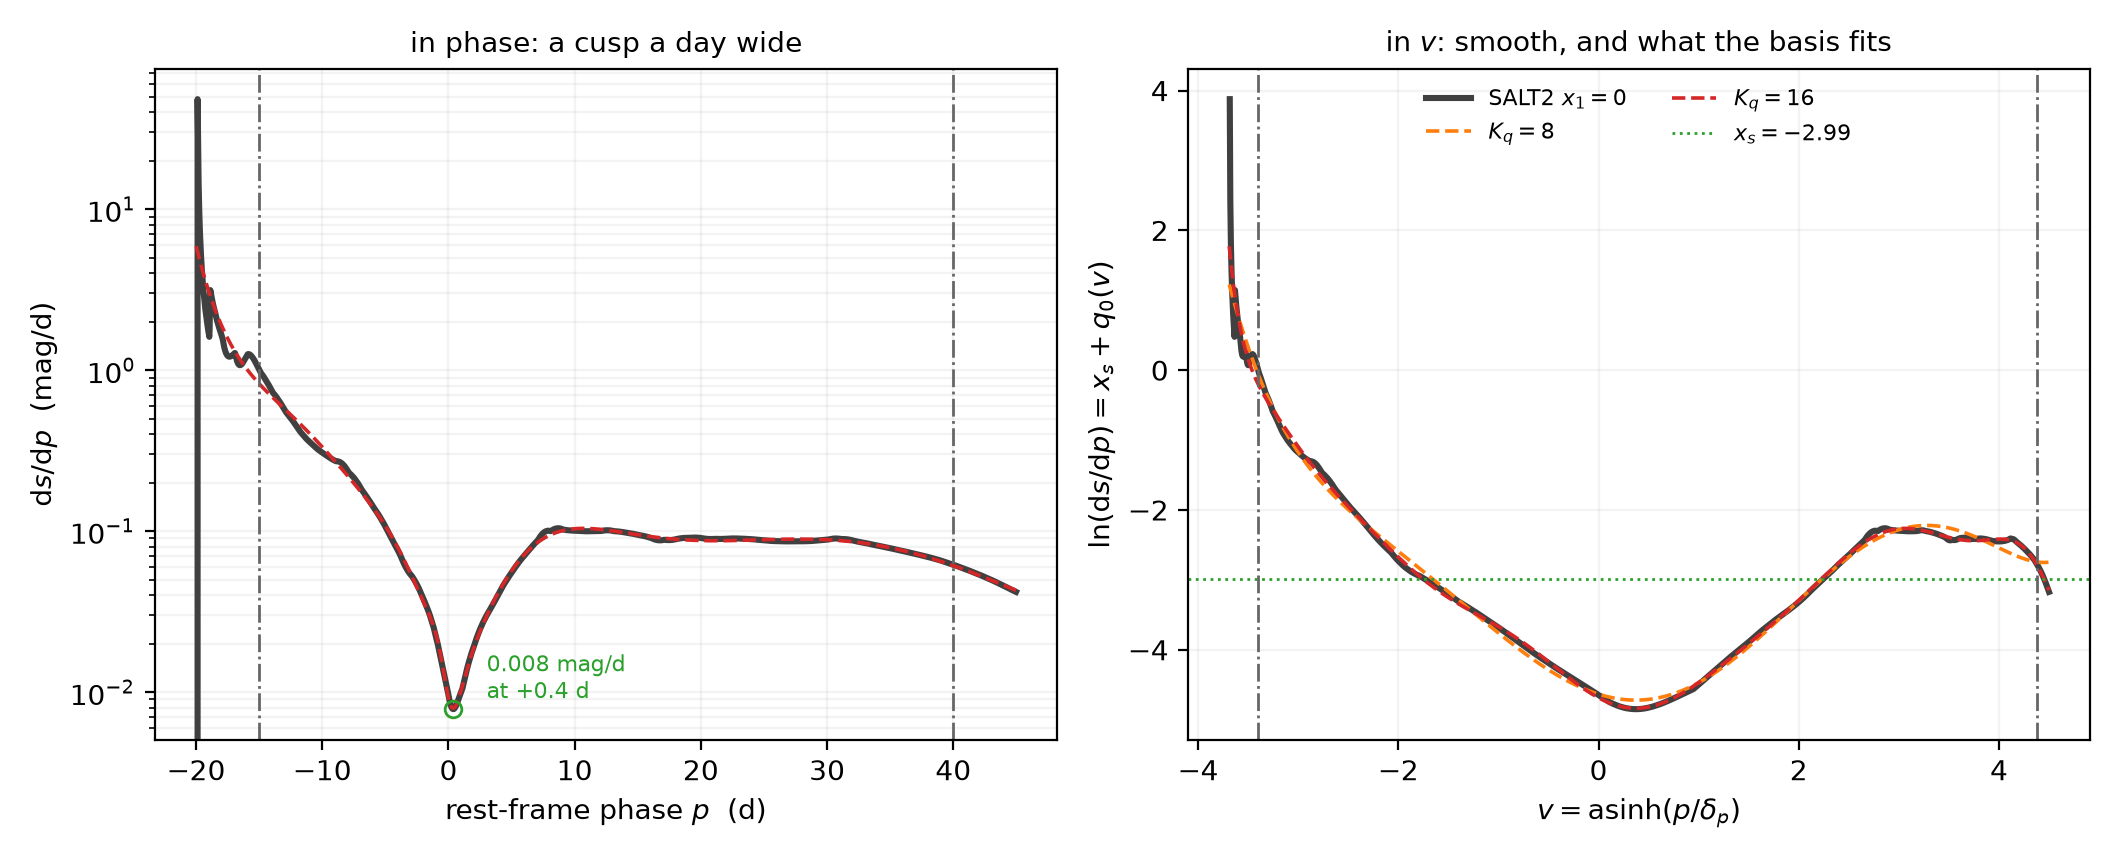
\includegraphics[width=\textwidth]{traversal-coordinates}
\caption{The two functions the population shares, each in the coordinate it is expanded
in. \emph{Left:} the turning $\turnzero(u) = \psi + \pi/2$ of a \salt\ track at $x_{1}=0$,
$c=0$, by \eqref{eq:cturn}, against $u = \mathrm{asinh}(\arc/\delta)$. Dash-dotted: the
arclengths the data window reaches, $\arc \in [-4.06, +3.18]$~mag, which is
$u \in [-7.39, +7.15]$. $\turnzero$ runs over $[-0.974, +2.556]$~rad there and is not
monotone, doubling back twice for a total variation of $5.33$~rad. Of its range, $38\%$ is
climbed inside $|\arc| < \delta = 5\times10^{-3}$~mag, a rise of $1.33$~rad over $1.03$~d of
phase, $1.9\%$ of the window, which the $\mathrm{asinh}$ opens to $12\%$ of the $u$ range. Dashed: the least-squares fit at
$K_{\psi} = 12$ and $24$, with maximum residual $0.32$ and $0.078$~rad over those
arclengths. \emph{Right:} the log rate, which by \eqref{eq:ctrav} \emph{is}
$x_{s} + q_{0}$, against $v$. In phase this quantity is a cusp --- $0.008$~mag/d at $+0.4$~d
against $1.0$ a fortnight earlier, a factor of $125$ in a feature a day wide --- and in $v$ it
is a smooth broad curve spanning $-4.85$ to $0.01$ over the data window, bottoming at
$v \simeq 0.37$ and flattening by $v \simeq 2.7$; $x_{s}$ is the dotted line, and $q_{0}$
oscillates about it with zero mean under $\int\dd v$. Dashed: the fit at $K_{q} = 8$ and
$16$, whose residuals in the log over the data window have root-mean-square $0.085$ and
$0.038$. The maximum residual barely moves between the two, $0.221$ against $0.202$, because
it lives in the five-day margins outside the data window and not in the body: the order is
set by the edges. Both coordinates do the same work --- they spend resolution where the
function turns, which in phase and in arclength is a vanishing fraction of the interval. The
track is an illustration of what the basis has to represent and is not fitted; nothing here
reaches a likelihood. Produced by \file{scripts/plot\_traversal.py}.}
\label{fig:coords}
\end{figure}

\paragraph{There is no gauge.} Every condition of the note's Eq.~(11) names a departure
mode, and this program has none: $\bar q_{1} = 0$ and $\langle q_{1},q_{1}\rangle = 1$ are
conditions on $q_{1}$, and $\langle q_{0},q_{1}\rangle = 0$ fixes $q_{0}$'s component along
it. So $\mathbf{b} = \tilde{\mathbf{b}}$ and $\mathbf{d} = \tilde{\mathbf{d}}$: no
normalization, no orthogonalization, and $G_{\arc}$, still built by the shared
\code{transformed data} include, is never read. $q_{0}$ and $\turnzero$ are functions the
data determine outright, with no coordinate freedom left to fix and no sign convention to
relabel afterwards.

Because $x_{s}$ is a constant in \eqref{eq:ctrav} and the basis carries no constant, the two
cannot trade: $x_{s}$ is the mean log rate and $q_{0}$ its shape, exactly and by
construction.

\subsection{Softening}
\label{sec:csoft}

Three places, all $C^{\infty}$, with
$\mathrm{softplus}(x,\epsilon) = \epsilon\log(1 + e^{x/\epsilon})$ and
$\mathrm{clamp01}(w,\epsilon) = \mathrm{softplus}(w,\epsilon) - \mathrm{softplus}(w-1,\epsilon)$:
\begin{align}
  w &= \frac{\phase - \phase_{\min}}{\phase_{\max} - \phase_{\min}} , &
  \hat\phase &= \phase_{\min} + (\phase_{\max}-\phase_{\min})\,\mathrm{clamp01}(w,\epsilon) ,\\
  \log\mathcal{T} &= -\left[\frac{e}{\epsilon_{t}}\right]^{2} , &
  e &= \mathrm{softplus}(-w, \tfrac{\epsilon_{t}}{10})
      + \mathrm{softplus}(w - 1, \tfrac{\epsilon_{t}}{10}) ,\\
  w_{\arc} &= \frac{\arc - \arc_{\min}}{\arcmax - \arc_{\min}} , &
  \hat\arc &= \arc_{\min} + (\arcmax - \arc_{\min})\,\mathrm{clamp01}(w_{\arc},\epsilon_{s}) .
\end{align}
The taper is evaluated at the \emph{unclamped} $w$, so it switches the flux off outside the
window rather than pinning it to the edge; the two clamps keep $\hat\phase$ and $\hat\arc$
inside the intervals the bases are defined on.

\subsection{Quadrature}

Both integrals, \eqref{eq:ctrav} and \eqref{eq:ccurve}, are taken by two-sided composite
Gauss--Legendre in the expansion coordinate: $m$ equal panels on $[lo, 0]$ and $m$ on
$[0, hi]$, $J$ points in each, so that zero is a panel edge and $\arc(0) = 0$,
$\curve(0) = 0$ hold by construction of the prefix table rather than up to a partial panel.
The change of variable carries its Jacobian,
\begin{equation}
  \dd\phase = \delta_{p}\cosh v\,\dd v , \qquad \dd\arc = \delta\cosh u\,\dd u ,
\end{equation}
and the stored weights are already multiplied by it. Panel integrals are summed once per
draw into a prefix table from zero outward; an epoch's remainder past its last edge is one
further fresh $J$-point panel. The panel index is found by a comparison loop, \code{floor}
not being castable to an integer in Stan when its argument depends on parameters.

\begin{figure}[htbp]
\centering
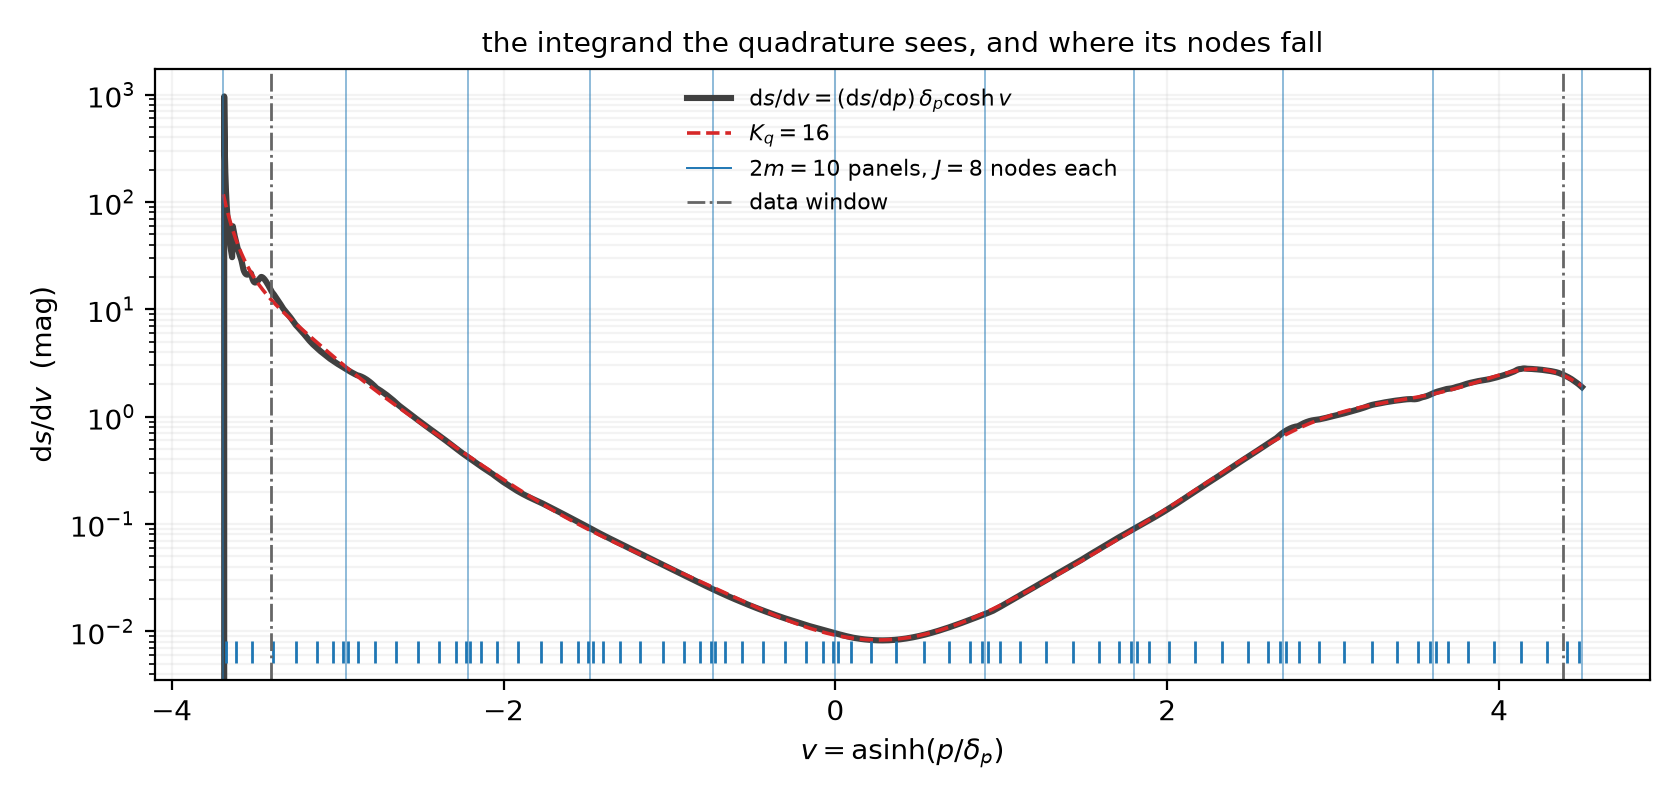
\includegraphics[width=0.86\textwidth]{traversal-quadrature}
\caption{The integrand of \eqref{eq:ctrav} as the rule meets it, and where the nodes fall.
Laying the panels in $v$ puts $16$ of the $80$ nodes in the two either side of zero --- one
per $0.11$ in $v$, which near the anchor is one per $0.11$~d, where the feature of
Figure~\ref{fig:coords} is. The same budget spread evenly in phase would give one node per
$0.8$~d and miss it. The Jacobian $\delta_{p}\cosh v$ tilts the integrand even though the
function of Figure~\ref{fig:coords} is nearly symmetric: it runs $0.008$ to $15.1$ over the
data window, so the integral's weight sits at large $|v|$ while its \emph{structure} sits at
the anchor. The leftmost panel, outside the data window, is where the integrand reaches
$10^{3}$ and the fit departs; that failure is confined to one panel and to phases no epoch
occupies. Produced by \file{scripts/plot\_traversal.py}.}
\label{fig:quad}
\end{figure}

\subsection{The likelihood}

In native flux, on the archive's errors alone:
\begin{equation}
  -2\ln\mathcal{L} = \sum_{i}
    \frac{(f_{i} - \hat f_{i})^{2}}{\sigma_{f,i}^{2}} .
\end{equation}
Nothing is converted to magnitudes and negative fluxes are ordinary measurements. The sum
is a \code{reduce\_sum} over supernovae, and $\hat f_{i}$ is the tapered flux, so an epoch
outside the window has its residual suppressed.

The variance used to carry a second term, $(k\sigma_{b}\hat f_{i})^{2}$ with
$k = 0.4\ln 10$ --- a fractional scatter with one fitted scalar per band --- and a
log-determinant beside it. Both are gone, and $\sigma_{g}, \sigma_{r}$ with them, since
with the second term removed they appear nowhere and a flat prior on a parameter the
likelihood does not see leaves the posterior improper. The log-determinant was not optional
while the variance depended on the parameters: $\sum(f-\hat f)^{2}/\sigma^{2}$ alone falls
monotonically in $\sigma$, so the fit would drive $\sigma_{b}$ to infinity. With
$\sigma_{f,i}$ data, $\sum\ln\sigma_{f,i}^{2}$ is an additive constant. Two consequences
for reading output: \code{lp\_sn} is now exactly $-\chi^{2}/2$, so a fit quality reads
straight off it, and a log-likelihood from this program is not comparable with one from a
program that kept the term until that constant is restored.

\subsection{Everything the program samples}

Seven quantities enter the forward map of \eqref{eq:cphase}--\eqref{eq:cflux}: the shared
$b_{0}, \mathbf{b}, \mathbf{d}$ and, per supernova,
$\Delta_{n}, x_{s,n}, m_{g,n}^{\max}, \colr_{n}$. Four are sampled as they stand; three
are assembled in \code{transformed parameters}, with $P_{0} = 1/\sqrt{v_{hi}-v_{lo}}$:
\begin{align}
  \Delta_{n} &= \code{delta\_t}[n] , &
  m_{g,n}^{\max} &= \code{m\_peak}[n] ,
    \label{eq:cmapA}\\
  x_{s,n} &= \code{x\_s}[n] , &
  b_{0} &= \code{b\_0} ,
    \label{eq:cmapB}\\
  \colr_{n} &= \code{c\_bar} + \code{c\_dev}[n] , &
  \code{x\_s\_tot}[n] &= x_{s,n} + b_{0}P_{0} ,
    \label{eq:cmapC}\\
  \mathbf{raw} &= R\,\code{w\_coef} , \qquad
  \mathbf{b} = \mathbf{raw}_{1:K_{q}-1} , &
  \mathbf{d} &= \mathbf{raw}_{K_{q}:K_{q}+K_{\psi}-2} .
    \label{eq:cmapD}
\end{align}
The coefficients are the one place where a sampled vector is not a physical quantity.
\code{w\_coef} has no meaning on its own: it is the vector the sampler moves on, and
\eqref{eq:cmapD} turns it into $\mathbf{b}$ and $\mathbf{d}$ through $R$, a fixed
$\bigl[(K_{q}{-}1)+(K_{\psi}{-}1)\bigr]^{2}$ matrix supplied as \code{data} and equal to the
identity unless a preconditioner has been built. Because $R$ is constant its Jacobian is
constant, so the change of variables alters no posterior --- it is a reparameterization
chosen to improve conditioning, and $\mathbf{b}$ and $\mathbf{d}$ are what the model means
either way. This is also why a rotation built at one $(K_{\psi}, K_{q})$ cannot be reused at
another: $R$'s dimension is fixed by the basis it was measured in.

Only the combination $x_{s,n} + b_{0}P_{0}$ reaches \eqref{eq:ctrav}, and the program forms
it once as \code{x\_s\_tot}; that is the exact gauge of the paragraph below, and the reason
$\xstretch$ alone is not a rate but a departure from one. In this program
$\mathbf{b} = \tilde{\mathbf{b}}$ and $\mathbf{d} = \tilde{\mathbf{d}}$ --- the note's
Eq.~(11) is vacuous here, every one of its conditions naming a departure mode --- so the
two names are kept only because \file{hier.stan} distinguishes them.

\begin{tabular}{llll}
\toprule
\multicolumn{4}{l}{\textbf{\code{parameters}} --- sampled; $162$ unconstrained coordinates} \\
 & shape & prior & reaches the model as \\
\midrule
\code{w\_coef}      & $(K_{q}{-}1) + (K_{\psi}{-}1)$ & below & $\mathbf{raw} = R\,\code{w\_coef}$ \\
\code{tau\_q}       & scalar $> 0$ & flat & scale of $\tilde{\mathbf{b}}$ \\
\code{tau\_psi}     & scalar $> 0$ & flat & scale of $\tilde{\mathbf{d}}$ \\
\code{alpha\_q\_m}  & scalar $> 0$ & $\mathrm{Exp}(1)$ & $\alpha_{q} - \frac12$ \\
\code{alpha\_psi\_m} & scalar $> 0$ & $\mathrm{Exp}(1)$ & $\alpha_{\psi} - \frac12$ \\
\code{b\_0}         & scalar, $b_{0}P_{0} \in [-20, 10]$ & flat & $q_{0}$'s degree-zero term \\
\code{x\_s}         & \code{sum\_to\_zero\_vector}$[N]$ & flat, walled at $\pm20$ & $x_{s}$, with $\langle x_{s}\rangle = 0$ \\
\code{c\_bar}       & scalar, $[-5, 5]$ & flat & mean of $\colr$ \\
\code{c\_dev}       & \code{sum\_to\_zero\_vector}$[N]$ & \textbf{none} & $\colr = \code{c\_bar} + \code{c\_dev}$ \\
\code{delta\_t}     & $N$, each in $[-3, 3]$ & flat & $\Delta$ \\
\code{m\_peak}      & $N$, each in $[5, 30]$ & flat & $\peakmag$ \\
\midrule
\multicolumn{4}{l}{\textbf{\code{transformed parameters}} --- built from the above, not sampled} \\
\midrule
\code{x\_s\_tot}    & $N$ & --- & $\xstretch + b_{0}P_{0}$, \eqref{eq:ctrav}'s exponent \\
\code{colr}         & $N$ & --- & $\colr$, by \eqref{eq:cmapC} \\
\code{b\_til}, \code{d\_til} & $K_{q}{-}1$, $K_{\psi}{-}1$ & --- & the two slices of $\mathbf{raw}$ \\
\code{b}, \code{d}  & $K_{q}{-}1$, $K_{\psi}{-}1$ & --- & $=\tilde{\mathbf{b}}, \tilde{\mathbf{d}}$; no gauge acts \\
\bottomrule
\end{tabular}

\medskip\noindent
$\mathbf{raw}$ is sliced into $\tilde{\mathbf{b}}$, the first $K_{q}-1$ entries, and
$\tilde{\mathbf{d}}$, the remaining $K_{\psi}-1$, and both carry the note's Eq.~(21) at the
geometric-mean pivot $\bar k = \exp[\overline{\ln k}]$:
\begin{equation}
  \tilde b_{k} \sim \mathcal{N}\!\left(0,\ \tau_{q}\,(k/\bar k_{q})^{-\alpha_{q}}\right) ,
  \qquad
  \tilde d_{k} \sim \mathcal{N}\!\left(0,\ \tau_{\psi}\,(k/\bar k_{\psi})^{-\alpha_{\psi}}\right) .
\end{equation}
Both are \emph{centred}: the data pin them, there being no gauge to remove their scale, so
$\tau_{q}$ and $\tau_{\psi}$ simply are the scales of $q_{0}$ and $\turnzero$ at a mid-range
mode. $R$ is a fixed \code{data} matrix over the coefficient block, the identity unless a
preconditioner has been built; being constant its Jacobian is constant, so it changes no
posterior.

\paragraph{Every prior here is flat.} Not one of the placement parameters carries a
distributional assumption. Where a bound is present it is a box, flat inside; where a mean
is named it is a free parameter, not a fitted population centre; and the two constrained
blocks, $\langle x_{s}\rangle = 0$ and $\langle\colr - \bar c\rangle = 0$, are gauge-fixings
rather than statements about how the objects are distributed. What a sum over realized
values asserts is nothing, where a normal population prior would assert Gaussianity.

\paragraph{$x_{s}$ and $b_{0}$: an exact gauge.} $q_{0}$ is expanded in Legendre degrees
$1$ to $K_{q}-1$ and therefore contains no constant, so $b_{0}P_{0}$ with
$P_{0} = 1/\sqrt{v_{hi}-v_{lo}}$ restores the degree-zero term. Only the sum
$x_{s,n} + b_{0}P_{0}$ reaches \eqref{eq:ctrav}'s exponent, so
$x_{s,n} \mapsto x_{s,n} + \epsilon$ with $b_{0} \mapsto b_{0} - \epsilon\sqrt{v_{hi}-v_{lo}}$
leaves every prediction identical: the degeneracy is \emph{exact}, and
$\sum_{n} x_{s,n} = 0$ fixes it at no cost, unlike $\Delta$'s near gauge below. What this
replaces --- a named mean $\bar s$ plus deviations --- is the same model relabelled; what it
buys is that $q_{0}$ is the population's log rate outright, mean included, rather than a
shape with its mean parked among the per-supernova parameters. $b_{0}$ is held outside the
block $R$ rotates for a specific reason: the same \code{traversal\_row} builds $q_{1}$, and
the note's Eq.~(11) requires $\bar q_{1} = 0$, so widening the slice to $[1\!:\!K_{q}]$ would
hand the departure mode a constant and break its gauge. It could not take the note's
Eq.~(21) in any case, $(k/\bar k)^{-\alpha}$ diverging at $k = 0$.

\paragraph{$\Delta$: a near gauge, confined rather than deleted.} A common shift of every
$\Delta$ is a shift of the phase origin, which $q_{0}$ --- a free function of $v$ ---
reshapes to absorb, so the population mean is pinned by the basis's finite flexibility and
not by the data. The fit says so directly: the per-supernova posterior standard deviation of
$\Delta$ is $0.359$~d, thirty independently measured offsets would put
$0.359/\sqrt{30} = 0.066$~d on their mean, and a hierarchical fit returned $0.344$~d, $5.2$
times larger. An earlier version of this program deleted that direction with
$\langle\Delta\rangle = 0$, at a measured cost of $1.96$ nats over $1568$ epochs
($1.25\times10^{-3}$ an epoch, the realized spread unmoved at $0.2989$~d, $\chi^{2}$ per
epoch moving from $5.229$ to $5.231$; the same comparison under the superseded likelihood
gave $2.19$ nats). The box confines it instead, so the fit finds its own phase origin, keeps
those nats, and leaves the $B$-to-$g$ offset in $\Delta$ rather than moving it into where
$q_{0}$ puts its minimum in $v$. The price is that the common mode is the long direction of
this block --- standard deviation $0.343$ and $0.437$ at $N = 30$ against a mean deviation
of $0.104$ and $0.109$, a ratio of $3.3$ and $4.0$, and $1.64$ at $N = 100$ --- and a
diagonal metric, assigning one scale per declared coordinate, has to straddle that ratio
where every coordinate mixes the two. $\Delta$ is the only one of the four where the ratio
exceeds unity; for $\peakmag$, $\colr$ and $x_{s}$ the common mode is the shorter direction.

\paragraph{What each bound is for.} Three directions do not fall away, and in each the
likelihood tends to a positive constant rather than to zero, so a flat prior over an
infinite range would not integrate. As $\peakmag \to +\infty$ the predicted flux vanishes and
the likelihood tends to $\exp(-\frac12\sum f^{2}/\sigma^{2})$. As $x_{s} \to -\infty$ the
rate vanishes, the track freezes at the anchor and the model is a constant light curve,
settling at $-4.83\times10^{6}$; as $x_{s} \to +\infty$ the rate diverges, every epoch is
driven into the arclength clamp, and the model is a constant light curve again at a
different constant, settling at $-2.93\times10^{6}$ --- the higher of the two, so the upward
tail is the more reachable. As $|\Delta|$ grows past about $100$~d every epoch leaves the
phase window, the softened clamp saturates, and the density reads $-156709.38$ at $300$~d
and $-156709.38$ at $1000$~d. Each box is sited far outside anything reachable and is a
statement about the archive rather than about supernovae: $\zp$ and $\peakmag$ are exactly
degenerate in \eqref{eq:cflux}, so the magnitude origin is a convention already fixed at
$\zp = 30$, in which $\peakmag = 30$ is a predicted flux of one archive unit against a
sample spanning $1.5\times10^{4}$ to $7.8\times10^{5}$; and $\pm3$~d is $8.6$ times the
largest $t_{0}$ uncertainty \ztf\ DR2 reports over the thirty.

$x_{s}$'s wall is written as a sampling statement and not as a declared bound, because
\code{sum\_to\_zero\_vector} admits no bounds --- \code{stanc} rejects the declaration
outright --- while \code{x\_s \textasciitilde\ uniform(-20, 20)} contributes exactly zero
inside the box and $-\infty$ outside. It is discontinuous, which costs nothing here: the
wall stands at some $270$ times the realized deviation standard deviation of $0.073$ and is
never met.

\paragraph{$\colr$ alone needs nothing.} Its deviations have no prior, and the reason is in
the forward map rather than in the statistics. Inside the sum-to-zero hyperplane some
component must run to $+\infty$, which drives that object's predicted $r$ flux up
exponentially, and a Gaussian-in-flux likelihood punishes that doubly exponentially: walked
out, the log density falls through $-4.67\times10^{6}$ at $t = 3$ and $-2.05\times10^{12}$
at $t = 10$ to $-\infty$, and on the least favourable ray available --- the object with five
$r$ epochs rising against the one with a hundred and thirteen falling --- faster still.
Colour is the one placement direction the map does not clamp, and clamping is exactly what
turns a runaway into a finite constant. The $\mathcal{N}(0,1)$ this replaces was shrinking by
$8.3\times10^{-4}$, so no number moves. An earlier version also had
$\colr \sim \mathcal{N}(0,1)$ centred on zero, which asserted a mean anchor colour of zero
where three fits put it at $+0.060 \pm 0.013$ at $N = 30$ and $+0.0597 \pm 0.0032$ at
$N = 100$; $\bar c$ carries it now, and the anchor conditions above record why the curve cannot.

At $K_{\psi} = 24$, $K_{q} = 16$ and $N = 30$ that is $38$ coefficients and $164$ named
values, four of them per supernova. Stan samples $162$ coordinates, not $164$: a
\code{sum\_to\_zero\_vector}$[N]$ is an orthogonal transform carrying $N-1$ unconstrained
coordinates, and there are two of them.

\subsection{The per-supernova parameters, one at a time}

Each of the four is asked three questions, and they are not alternatives: a parameter can
answer yes to more than one, and the answers call for different devices. \emph{Is there an
exact degeneracy} --- a direction along which the likelihood is exactly constant? Then a
constraint is right, because it deletes a coordinate that carries no information.
\emph{Is there a near one}, where the likelihood is almost constant and only the basis's
finite flexibility pins it? A constraint is still right, but it costs something and the cost
is measured rather than assumed. \emph{Are the tails flat} --- does the likelihood tend to a
positive constant at infinity? Then a bound or a proper prior is needed, and a constraint
does not supply one. The three sum-to-zero blocks here settle that last point by example:
under a flat prior one of them is proper and two are not.

A fourth question is bookkeeping and not inference. Where a mean is identified, writing it
as a named scalar plus deviations summing to zero is a reparameterization --- the same
posterior over the same $N$ coordinates --- which makes the common mode one coordinate
instead of $N$. That is all $\bar s$ and $\bar c$ are.

\paragraph{$\peakmag$: an exact gauge, already fixed.} It is the only one of the four with
an exact degeneracy. Predicted flux depends on $\peakmag$ and $\zp$ only through
$\peakmag - \zp$, so a common shift of every $\peakmag$ against $\zp$ changes nothing, and
pinning $\zp = 30$ is what fixes it --- the gauge is spent before the fit begins, which is
why no constraint appears on $\peakmag$ here. Its one flat tail is the faint one: as
$\peakmag \to +\infty$ the predicted flux vanishes and the likelihood tends to
$\exp(-\frac12\sum f^{2}/\sigma^{2})$, small but positive. The box closes it, and because
the magnitude origin is already a convention the bound inherits that convention rather than
asserting anything. The prior it replaced,
$\mathcal{N}(m_{g}^{\mathrm{bright}}, 1)$, was shrinking by $2.7\times10^{-4}$ to
$3.5\times10^{-3}$ and reading the same photometry the likelihood reads.

\paragraph{$\colr$: no gauge, and the only one that needs no prior.} $\curve(0) = 0$ fixes
the curve's anchor in both components, so $\colr$ \emph{is} the $g-r$ colour at the anchor
and its mean is identified: the fits put it at $+0.060 \pm 0.013$ over thirty objects and
$+0.0597 \pm 0.0032$ over a hundred, nineteen standard deviations from zero. Naming $\bar c$
is therefore bookkeeping, not gauge-fixing. What is unusual is the tails. Inside the
sum-to-zero hyperplane some component must run to $+\infty$, which drives that object's
predicted $r$ flux up exponentially, and a Gaussian-in-flux likelihood punishes that doubly
exponentially: walked out, the log density falls through $-4.67\times10^{6}$ at $t = 3$ and
$-2.05\times10^{12}$ at $t = 10$ to $-\infty$. Checked on the least favourable ray
available, the object with five $r$ epochs rising against the one with a hundred and
thirteen falling, it diverges faster still, since the rising object is the punished one and
a single epoch suffices. A flat prior on the deviations is proper on its own.

\paragraph{$\Delta$: a near gauge, confined.} The degeneracy with $q_{0}$'s phase origin is
approximate, not exact --- deleting it with $\langle\Delta\rangle = 0$ cost $1.96$ nats ---
so $\Delta$ is boxed rather than constrained and the mean floats inside the box. It also has
flat tails at both ends, the phase clamp saturating the model's dependence on $\Delta$
altogether, so the bound is doing two jobs at once: confining the near gauge and supplying
propriety. It is the only one of the four needing both.

\paragraph{$\xstretch$: an exact gauge, fixed.} With $b_{0}$ restoring $q_{0}$'s
degree-zero term, only $x_{s,n} + b_{0}P_{0}$ reaches the exponent, so the shift between
them is an exact symmetry and $\langle\xstretch\rangle = 0$ removes it for nothing. Both
tails are flat, which Section~5 of the note until recently recorded for only one of them,
and the deviations inherit no propriety from their constraint: a ray inside the hyperplane
sends one object to each plateau and settles at $-2.47\times10^{5}$. Hence the wall.

\paragraph{Why $\colr$ differs.} Both constrained blocks are the same kind of object and
behave differently, and the reason is in the forward map rather than in the statistics.
Colour has no clamp, so a runaway direction drives a predicted flux to infinity and the
likelihood kills it. Arclength and phase are both clamped, so every runaway saturates into a
constant light curve instead, which is finite and therefore flat. The question to ask of any
future constrained block is which of those two it is: whether the forward map clamps that
direction or lets it diverge.

\subsection{What it reports}

Per draw: $\alpha_{q}$ and $\alpha_{\psi}$; $\curv(0) =
\turnzero'(0)/\delta$, the turning rate at the anchor; $\arc$ at both ends of the data window
for every supernova, against which the declared interval is checked; the fractions of epochs
tapered and arclength-clamped; and $\ln\mathcal{L}$ per supernova, from which a per-epoch
figure of merit follows. No sign flags and no relabeled copies: with no departure mode there
is no sign freedom to record.

\section{The declared constants}
\label{sec:constants}

From \file{src/dgsn/stan/data.py}. The third column is what
\file{model-definition.tex} states.

\begin{tabular}{llll}
\toprule
 & code & note & \\
\midrule
$\delta$, Eq.~(14)        & $5\times10^{-3}$ mag & $3\times10^{-4}$ mag & \textcolor{red}{differs} \\
$\delta_{p}$, Eq.~(12)    & $1.0$ d & $1.0$ d & \\
$[\phase_{\min}, \phase_{\max}]$ & $[-20, +45]$ d & $[-20, +45]$ d & \\
$[\arc_{\min}, \arcmax]$, Section~3 & $[-8, +8]$ mag & $[-12, +6]$ mag & \textcolor{red}{differs} \\
gauge span, Eq.~(11)      & $[-6, +5]$ mag & $[-6, +5]$ mag & \\
$\epsilon$                & $0.01$ & $0.01$ & \\
$\epsilon_{t}$            & $0.02$ & $0.02$ & \\
$\epsilon_{s}$            & $10^{-3}$ & $10^{-3}$ & \\
$\zp$                     & $30$ & $30$ & \\
$m$, Section~5.1          & $5$, so $M = 10$ & $10$, so $M = 20$ & \textcolor{red}{differs} \\
$J$                       & $8$ & $8$ & \\
$K_{\psi}, K_{q}$         & $24, 16$ & $24, 16$ & \\
$\bar x_{s}$, Eq.~(22)    & kept for \file{single\_sn.stan} only & withdrawn & \\
\bottomrule
\end{tabular}

\section{Where one expression spans several statements}
\label{sec:fused}

These are not divergences. They are the places where the code evaluates in one line what the
note states in two or three, so that reading one section of the note alone can set a wrong
expectation.

\paragraph{The two integrals.} Eq.~(10) and Eq.~(5) are written as integrals in $\dd\phase$
and $\dd\arc$. Eqs.~(12) and (14) give the coordinates. The Jacobians
$\dd\phase = \delta_{p}\cosh v\,\dd v$ and $\dd\arc = \delta\cosh u\,\dd u$ appear only in
Section~5.1, in prose, where the subject is quadrature accuracy. A reader of Section~2.3
meets the bases and the gauge with no measure in view but $\dd v$ and $\dd u$, which is how
the gauge asymmetry of Section~\ref{sec:gauge} survives: Section~2.3 argues carefully for
$\dd\arc$ over $\dd u$ for the turning, specifies the traversal in $\dd v$ on the facing
page, and the fact that Eq.~(10) carries $\delta_{p}\cosh v$ is four sections away.

\paragraph{Two of Eq.~(11)'s four conditions are free.} $\bar q_{0} = \bar q_{1} = 0$ hold
because \code{traversal\_row} drops the constant Legendre term. The code imposes the other
two. Counting four conditions suggests four things to check; there are two.

\paragraph{The anchor conditions.} $\turnzero(0) = \turnone(0) = 0$ of Eq.~(9), and
$\arc(0) = 0$ and $\curve(0) = 0$, are all structural: the first pair from the shift in
\code{turning\_row}, the second pair from the prefix table being laid outward from zero so
that zero is a panel edge. None is a constraint the sampler respects; all hold to rounding.

\section{Where the code and the note differ}
\label{sec:differ}

\paragraph{Three constants.} $\delta$ is seventeen times larger than the note states, the
arclength interval is $[-8, +8]$ rather than $[-12, +6]$, and the quadrature uses half the
panels. The first two were changed together when the basis was re-scaled onto the data; the
third was taken as free on an accuracy budget. All three are recorded with their
measurements in \file{docs/model-note-backlog.md}, and none has been written back into
Sections~2.3 or~3.

\paragraph{Three programs the note does not describe.} \file{hier\_nomode.stan} removes
$\shapeturn\turnone$ from Eq.~(9) of \file{model-definition.tex}, and
\file{hier\_common.stan} removes $x_p q_{1}$ from Eq.~(10) as well, taking both gauges and
both sign conventions with them --- Section~\ref{sec:nested}. \file{jacobian.stan} exists
only to supply $J$ for the preconditioner. None is a divergence in the sense of
contradicting the note: each is a strictly smaller model, built to measure what the note's
own terms are worth, and the note's model is \file{hier.stan}.

\paragraph{One parameter the note does not describe.} The rotation $R$ is a
reparameterization and so changes nothing inferentially, but the note's
Section~5 does not mention it, and a reader of \file{hier.stan} meets it in the
\code{data} block.

\paragraph{Orders in use.} The constants declare $K_{\psi}, K_{q} = 24, 16$, but every fit
run so far has passed $(12, 8)$ or $(24, 16)$ on the command line. The note's grid over
$K_{\psi}$ and $K_{q}$ is still outstanding.

\end{document}
